\documentclass[]{article}

\usepackage[margin=1.0in]{geometry}

\usepackage{amsmath}  % assumes amsmath package installed
\usepackage{amssymb}  % assumes amsmath package installed
\usepackage{graphicx}
\usepackage{todonotes}
\usepackage{float}
\usepackage{lipsum}

\usepackage[framed,numbered,autolinebreaks,useliterate]{mcode}
%\usepackage{filecontents}
\usepackage{pdfpages}
\usepackage{subfig}

% for subfigures
\usepackage{caption}
\usepackage{subcaption}

%
%opening
\title{Probabilistic Algorithms for Aerospace Autonomy\\ASEN 6519 - Project Update\\MLESAC \& Othrogonal Distance Regression:\\ Velocity Profile Parameter Estimation}
\author{Carl Stahoviak}

\begin{document}

\maketitle

%\begin{abstract}
%
%\end{abstract}

\tableofcontents
%\listoftodos[Notes]

\newpage
\section{Application and Context}

\subsection{Radar Doppler Velocity}

The doppler velocity measurement produced by the radar for a given target is equal to the magnitude of the projection of the relative velocity vector onto the line $\mathbf{r}$ defined between sensor origin and the target location, i.e. radar doppler is a measure of how the sensor and the target are moving relative to one another along the line-of-sight between the sensor and the target. Positive doppler velocities are produced when the sensor and target are moving towards each other, and negative doppler velocities are produced when the sensor and target are moving away from away from one another. In general, the doppler velocity of target $i$ can be expressed as 

\begin{equation}
	v_{r,i} = \text{comp}_{\mathbf{r}} \mathbf{v}_{\text{rel}}
	\label{eqn:projection_rel}
\end{equation}

We will assume that every target in the scene is stationary, and that only the sensor platform is moving. One expected benefit of the MLESAC implementation is a means by which dynamic agents in the environment can be effectively handled and treated as outliers in the estimation of the body-frame velocity of the sensor platform.Assuming target $i$ is stationary relative to the sensor platform and that the sensor is aligned with the body-frame axes, Eqn. \ref{eqn:projection_rel} can be re-written as

\begin{equation}
	v_{r,i} = \text{comp}_{\mathbf{r}} \mathbf{v}^b
	\label{eqn:projection_body}
\end{equation}

where $\mathbf{v}^b$ denotes the body-frame velocity of the sensor platform. Motion in the plane normal to $\mathbf{r}$ is completely unobservable by the radar, rendering the $v_t$ component of the target-frame velocity unobservable and thus the body-frame velocity of the platform cannot be solved for a single target.

Rewriting Eqn. \ref{eqn:projection_body} we can express the doppler velocity $v_{r,i}$ as a function of the body-frame velocities of the sensor platform $[v_x, v_y]^T$ and the angular location of the target $\theta_i$

\begin{equation}
\begin{aligned}
	v_{r,i} &= \text{comp}_{\mathbf{r}} \mathbf{v}_x^b + \text{comp}_{\mathbf{r}} \mathbf{v}_y^b  \\
			&= v_x \cos \theta_i + v_y \sin \theta_i \\
			&= v \cos \phi \cos \theta_i + v \sin \phi \sin \theta_i \\
			&= v \cos( \phi - \theta_i)
	\end{aligned}
	\label{eqn:generative_model}
\end{equation}

The 2D body-frame velocity estimation problem can now be posed an an over-determined non-linear system of equations where each unique equation corresponds to a target $i = 1,\ldots,n$ in the scan.

\begin{equation}
	\begin{bmatrix} v_{r,1}\\ v_{r,2}\\ \vdots\\ v_{r,n} \end{bmatrix} = 
	\begin{bmatrix} \cos \theta_1 & \sin \theta_1 \\ \cos \theta_2 & \sin \theta_2 \\ \vdots & \vdots \\ \cos \theta_n & \sin \theta_n \end{bmatrix}
	\begin{bmatrix} v_x \\ v_y  \end{bmatrix}
	\label{eqn:overdetermined}
\end{equation}

Equation \ref{eqn:overdetermined} has a unique solution for two targets ($i,j$) with distinct angular locations, $\theta_i \neq \theta_j$, and regression analysis can be used to determine the parameters, $v_x$ and $v_y$.


\section{Probabilistic Model}

\subsection{Radar Doppler Generative Model}

The generative model for this problem is described mathematically by Eqn. \ref{eqn:overdetermined}. Graphically, this model looks similar to that of the latent variable model of homework 2, where the latent variables are the \emph{true} values of $\bar{\theta}_i$ and $\bar{v}_{r,i}$.

\begin{figure}[H]
	\centering
	\captionsetup{justification=centering}
	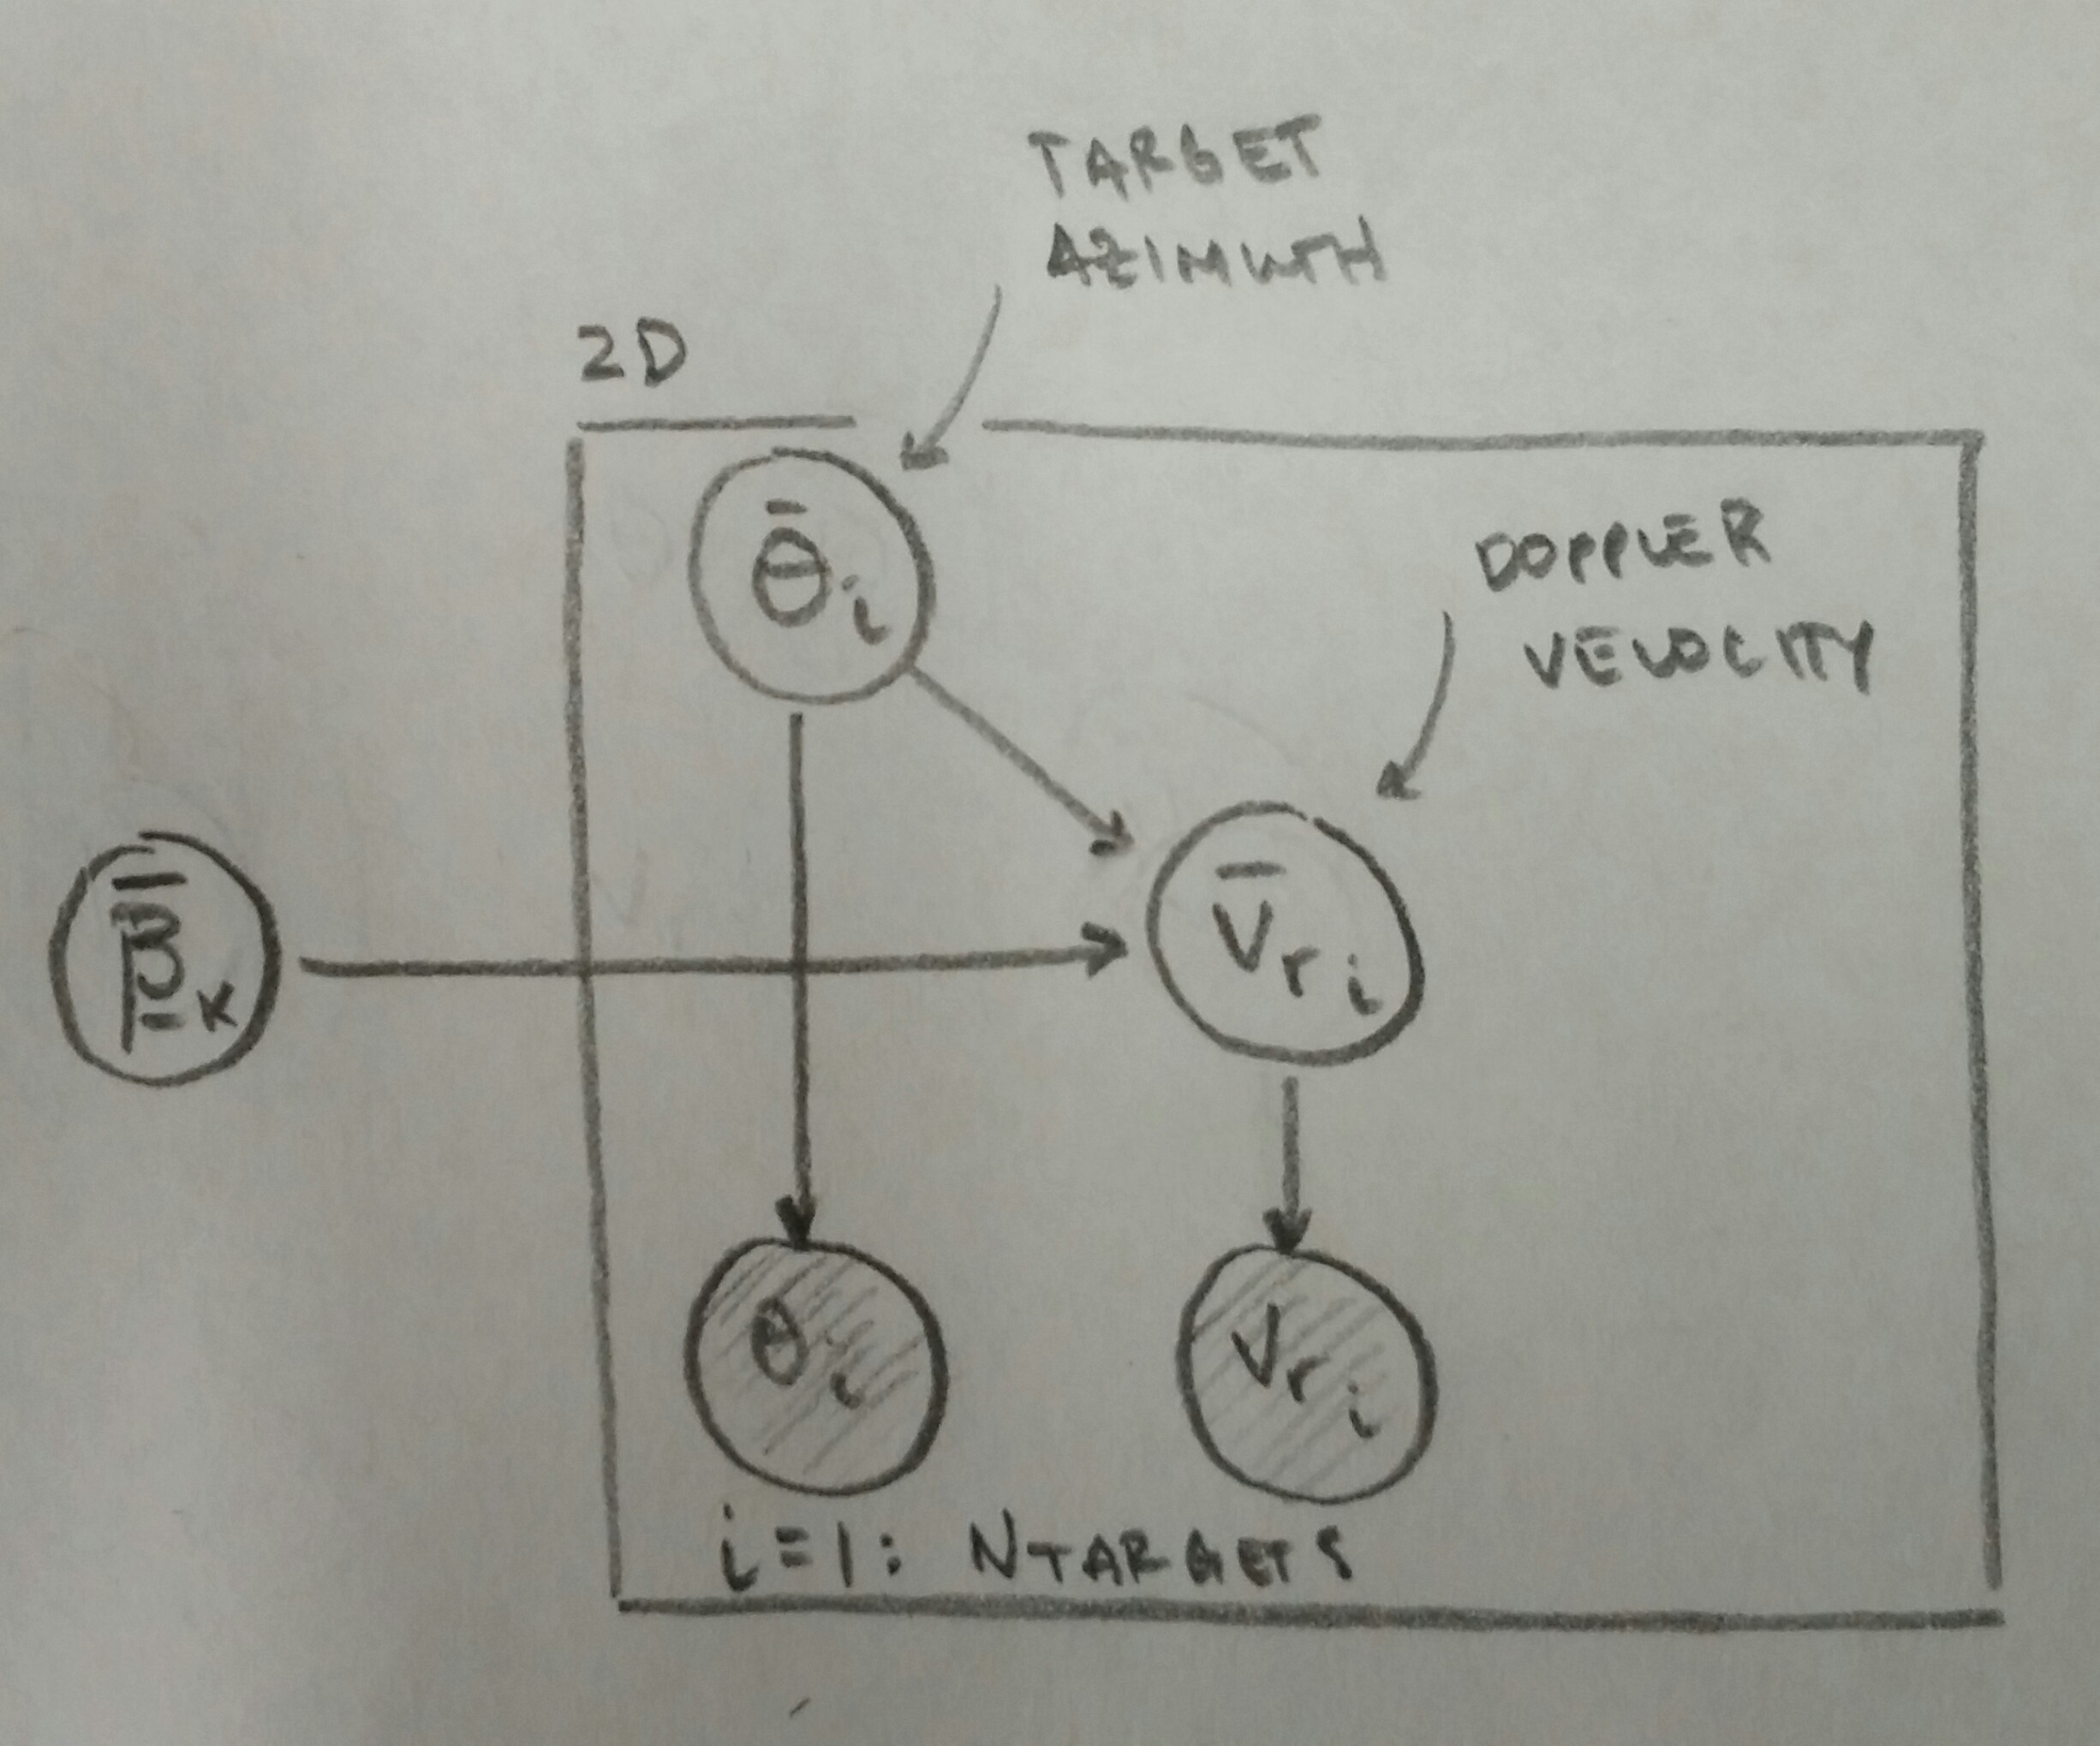
\includegraphics[width=.50\textwidth]{graphicalmodel.jpg}
	\caption{\small 2D radar doppler velocity generative model}
\end{figure}

In order to define the measurement model, let us assume that $X_i$ and $Y_i$ are observed random variables with underlying true values $x_i$ and $y_i$, with random zero-mean Gaussian error $\epsilon_i \sim \mathcal{N}(0,\sigma_x)$ and $\delta_i \sim \mathcal{N}(0,\sigma_y)$, respectively, such that

\begin{equation}
	\begin{aligned}
	X_i = x_i - \delta_i \\
	Y_i = y_i - \epsilon_i
	\end{aligned}
\end{equation}

The measurement model for $y_i$ can now be defined in general terms as a function of both $x_i$ and the parameter set $\beta$

\begin{equation}
	y_i = f(x_i;\boldsymbol{\beta})
\end{equation}

or 

\begin{equation}
	Y_i = f(X_i + \delta_i;\boldsymbol{\beta}) - \epsilon_i
\end{equation}


The radar doppler measurement associated with a given target in the scan is a function of both the target's angular location $X_i = \theta_i$ and the sensor platform body-frame velocity given by the parameter set to be estimated $\boldsymbol{\beta} = [v_x, v_y]^T$.

\begin{equation}
	v_{r,i} = f(\theta_i + \delta_i;\begin{bmatrix} v_x \\ v_y \end{bmatrix}) - \epsilon_i = v_x \cos(\theta_i + \delta_i) + v_y \sin(\theta_i + \delta_i) - \epsilon_i
\end{equation}



\section{Objectives}

The following objectives are listed in terms of complexity of implementation:

\begin{enumerate}
	\item Implement 'brute-force' parameter estimation in which the parameter set $\boldsymbol{\beta} = [v_x,v_y]^T$ is estimated for every pair of targets ($i,j$) in the scan. The estimate of $\boldsymbol{\beta}$ can be given as a weighted maximum likelihood estimate, where the weighting scheme can take into account the normalized target intesity values (proportional to the radar cross section of the target).
	\item Implement Maximum Likelihood Estimation Sample and Consensus (MLESAC) for parameter estimation
	\item Implement Orthogonal Distance Regression (ODR) for parameter estimation
\end{enumerate}

\subsection{Brute Force Parameter Estimation}

The 'brute force' parameter estimation approach solves the uniquely-determined problem for every pair of targets ($i,j$) in the scan such that $\theta_i \neq \theta_j$.

\begin{equation}
	\begin{bmatrix} v_x \\ v_y  \end{bmatrix}_{ij} = 
	\begin{bmatrix} \cos \theta_i & \sin \theta_i \\ \cos \theta_j & \sin \theta_j \end{bmatrix}^{-1}
	\begin{bmatrix} v_{r,i}\\ v_{r,j}\\  \end{bmatrix}	
\end{equation}

Due to binning in range, angle and doppler space, it will be almost guaranteed that some subset of the targets in a particular scan satisfy $\theta_i = \theta_j$ . Computationally, this will cost $(n-1)n/2$ calculations per scan. After discarding for outliers in the parameter estimate (2$\sigma$ outliers perhaps), the parameter estimate can be given as

\begin{equation}
	\begin{bmatrix} v_x \\ v_y \end{bmatrix}^* = \sum_{i=1}^{n-1} \sum_{j=i+1}^n w_{ij} \begin{bmatrix} v_x \\ v_y  \end{bmatrix}_{ij} \bigg/\sum_{i=1}^{n-1} \sum_{j=i+1}^n w_{ij}
\end{equation}

where a weighting scheme that takes into consideration the target's returned signal intensity value may be used.
	

\subsection{MLESAC Parameter Estimation}

Random Sample and Consensus (RANSAC) is an iterative method to estimate the parameters of a mathematical model from a set of observed data that contains outliers, when outliers are to be accorded no influence on the values of the estimates. In this sense, it can also be interpreted as an outlier detection method. It is a non-deterministic algorithm that seeks to estimate the parameter set by maximizing the number of data points ascribed to the inlier set

Maximum Likelihood Estimation Sample and Consensus (MLESAC) \cite{MLESAC} adopts the same sampling strategy as RANSAC, but determines a parameter estimate that maximizes the data log-likelihood rather than maximizing the number of data points in the inlier set.

Let us revisit the assumption that $\epsilon_i$ is a zero-mean Gaussian random variable, $\epsilon_i \sim \mathcal{N}(0,\sigma_x)$. In general, the log of the likelihood function is given by

\begin{equation}
	\log P(\mathbf{X} \vert \mu, \sigma^2) = \log \prod_{i=1}^N \mathcal{N}(x_i \vert \mu, \sigma^2)	
\end{equation}

For the case of the radar doppler generative model, the data log-likelihood function can be expressed as

\begin{equation}
	\log P(\mathbf{v_r} \vert \boldsymbol{\beta}) = \log \prod_{i=1}^N \frac{1}{(2\pi\sigma_{v_r}^2)^{1/2}} \cdot \exp \bigg\lbrace -\frac{1}{2\sigma_{v_r}^2} \big( f(\theta_i;\boldsymbol{\beta}) - v_{r,i} \big)^2 \bigg\rbrace
\end{equation}

where $\epsilon_i = f(\theta_i;\boldsymbol{\beta}) - v_{r,i}$. What follows is a derivation of the final form of the data log-likelihood, $\log P(\mathbf{v_r} \vert \boldsymbol{\beta})$.

\begin{equation}
	\log \bigg\lbrack \left( \frac{1}{(2\pi\sigma_{v_r}^2)} \right)^{N/2} \cdot \left( \exp \bigg\lbrace -\frac{1}{2\sigma_{v_r}^2} \epsilon_1^2 \bigg\rbrace \times \cdots \times \exp \bigg\lbrace -\frac{1}{2\sigma_{v_r}^2} \epsilon_N^2 \bigg\rbrace  \right) \bigg\rbrack
\end{equation}

\begin{equation}
	\frac{N}{2} \log \left( \frac{1}{(2\pi\sigma_{v_r}^2)} \right) + \log \bigg\lbrack \exp \bigg\lbrace -\frac{1}{2\sigma_{v_r}^2} \epsilon_1^2 \bigg\rbrace \times \cdots \times \exp \bigg\lbrace -\frac{1}{2\sigma_{v_r}^2} \epsilon_N^2 \bigg\rbrace \bigg\rbrack
\end{equation}

\begin{equation}
	\frac{N}{2} \left( \log(1) - \log (2\pi\sigma_{v_r}^2) \right) + \log \bigg\lbrack \exp \bigg\lbrace -\frac{1}{2\sigma_{v_r}^2} \epsilon_1^2 \bigg\rbrace \bigg\rbrack + \cdots + \log \bigg\lbrack \exp \bigg\lbrace -\frac{1}{2\sigma_{v_r}^2} \epsilon_N^2 \bigg\rbrace \bigg\rbrack
\end{equation}

\begin{equation}
	-\frac{N}{2} \log(2\pi) - \frac{N}{2} \log(\sigma_{v_r}^2) - \frac{1}{2\sigma_{v_r}^2} \sum_{i=1}^N \epsilon_i^2
\end{equation}

And finally disregarding the first two constant terms, we can express the data log-likelihood as

\begin{equation}
	\log P(\mathbf{v_r} \vert \boldsymbol{\beta}) = - \frac{1}{2\sigma_{v_r}^2} \sum_{i=1}^N \big( f(\theta_i;\boldsymbol{\beta}) - v_{r,i} \big)^2
\end{equation}

For the case of normally distributed, zero-mean errors, maximizing the data log-likelihood results in minimizing the ordinary least-squares (OLS) problem. To evaluate the performance of the MLESAC algorithm, a set of simulated radar doppler measurements are generated with outliers. The MLESAC solution and the OLS solution are compared against the true velocity profile. Uncertainty in doppler and azimuth measurements are expressed as $\sigma_{v_r} = 0.044$ m/s and $\sigma_{\theta} = 2.36$ deg.

\begin{figure}[H]
	\centering
	\subfloat[MLESAC inlier and outlier classified data ]{{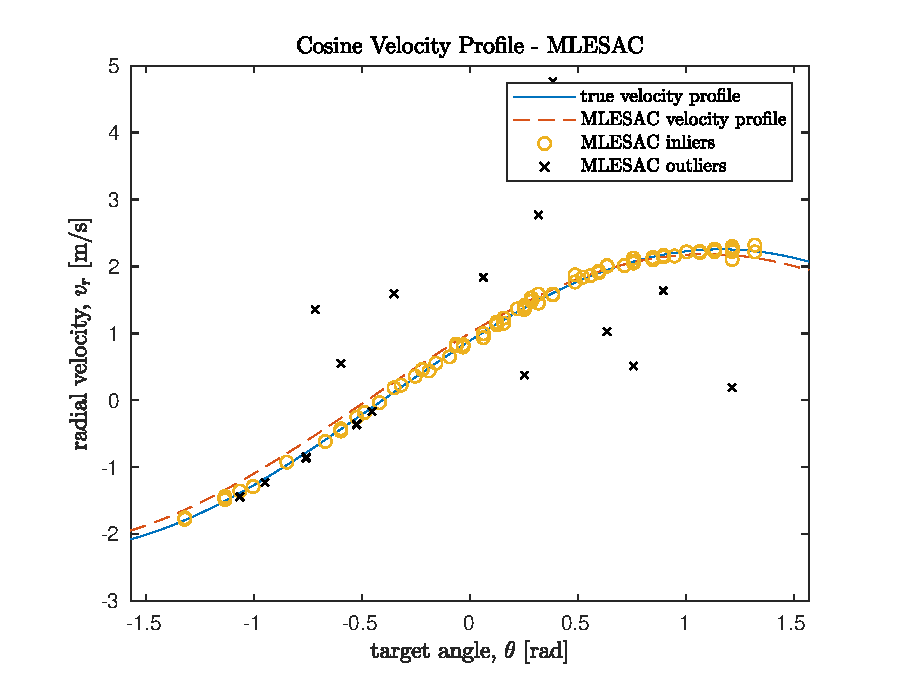
\includegraphics[width=7.75cm]{figures/mlesac_profile.eps} }}
	\quad
	\subfloat[MLESAC data log-likelihood]{{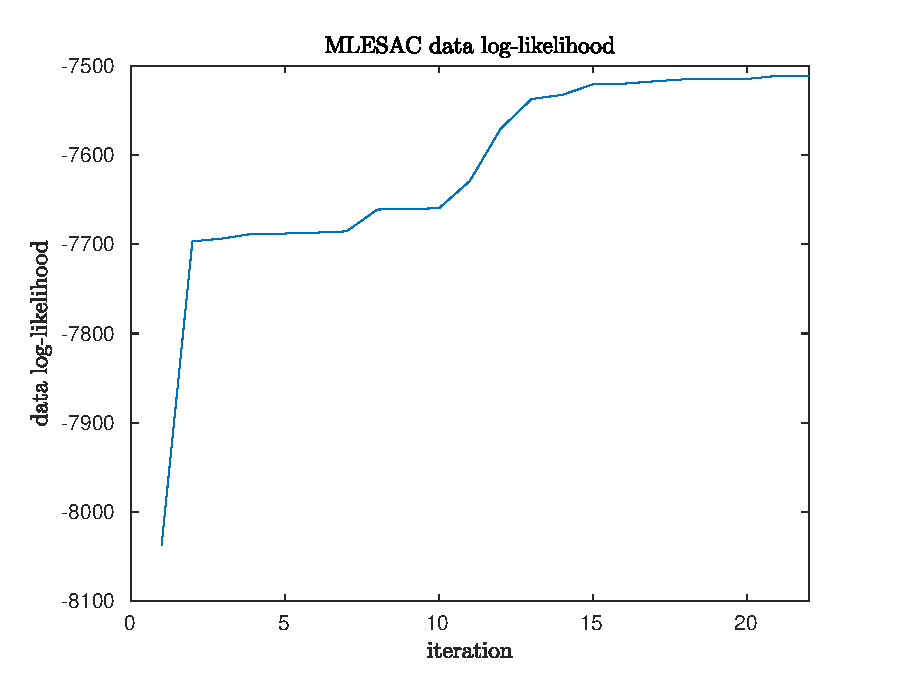
\includegraphics[width=7.75cm]{figures/mlesac_log_likelihood.eps} }}%
	\caption{MLESAC velocity profile estimation}
	\label{fig:example}
\end{figure}

\subsection{Orthogonal Distance Regression Parameter Estimation}

The final step in the body-frame velocity estimation problem problem is the implementation of Orthogonal Distance Regression (ODR) \cite{ODR_1987} \cite{ODRPACK95} on the MLESAC inlier set. ODR is an error-in-variables regression technique that accounts for errors in the measured (explanatory) variables ($\theta_i, v_{r,i}$) in the estimation of the parameter vector $\beta=[v_x,v_y]^T$. In general, the observation model can be stated as
\begin{equation}
	y_i + \epsilon_i = f(x_i;\beta)
\end{equation}

And for the case of 2D radar as
 
\begin{equation}
	v_{r,i} = f(\theta_i; [v_x, v_y]^T) = v_x \cos \theta_i + v_y \sin \theta_i 
\end{equation}

In Ordinary Least Squares, it is assumed that $x_i = \theta_i$ is known exactly and $y_i = v_{r,i}$ is observed with error $\epsilon_i$. OLS can be interpreted as minimizing the sum of the squares of the vertical distances from the observed data points to the curve $y = f(x;\beta)$.

\begin{equation}
	 \min_{\beta} \sum_{i=1}^n \epsilon_i^2 
\end{equation}

ODR operates under the assumption that their is error in both the measurement of $x_i$ and $y_i$, given by $\epsilon_i$ and $\delta_i$ respectively where $\epsilon_i \sim \mathcal{N}(0,\sigma_y)$ and $\delta_i \sim \mathcal{N}(0,\sigma_x)$ =. The observation model is then re-written as:

\begin{equation}
	 y_i + \epsilon_i = f(x_i + \delta_i;\beta) 
\end{equation}

and ODR can be interpreted as minimizing the sum of the squares of the orthogonal distances of the observed data points to the curve $y = f(x;\beta)$.

\begin{equation}
	 \min_{\beta, \delta} \sum_{i=1}^n \epsilon_i^2 + \delta_i^2 
\end{equation}


\bibliographystyle{ieeetr}	% We choose the "plain" reference style
\bibliography{references}	% Entries are in the "references.bib" file

\end{document}

